% !Mode:: "TeX:UTF-8"
\documentclass[a4paper,12pts]{article}

%\usepackage[polish]{babel}
\usepackage{polski}
\usepackage{fontspec}
\setmainfont{Calibri}

\linespread{1.15}

\usepackage{caption}
\captionsetup{%
	font={footnotesize},
	labelfont={bf}
}

\usepackage{anysize}
\usepackage{geometry}
\usepackage{graphicx}

\sloppy

\begin{document}
	\thispagestyle{empty}
	\begin{flushleft}
		Wydział Elektrotechniki, Automatyki, Informatyki i Inżynierii Biomedycznej \\
		Informatyka, rok II \\
		Zespół numer 3 \\
		Piotr Kucharski \\
		Dominik Zabłotny \\
		\vspace*{\fill}
		%-----------NUMER CWICZENIA--------%
		{\large \textbf{Sprawozdanie z ćwiczenia nr 0} } \\
		%-----------TEMAT ĆWICZENIA--------%
		Wyznaczanie przyspieszenia ziemskiego za pomocą wahadła matematycznego.		
		\vfill	
		%-----------DATA-------------%
		11 października 2017r
	\end{flushleft}
	
	\newpage
	
%--------------------------------------------------------------------------------------------------------------
	
	\section{Cel ćwiczenia}
	
%--------------------------------------------------------------------------------------------------------------
	
	\section{Wykonanie ćwiczenia}
	
%--------------------------------------------------------------------------------------------------------------
	
	\section{Opracowanie danych pomiarowych}
	
	\subsection{Przyspieszenie grawitacyjne dla stałej długości nici wahadła}
	Zmierzone wielkości zapisano w tabeli \ref{Tabela1}, gdzie uwzględniono czas wykonania $k$ okresów w czasie $t$ oraz wyliczono odpowiednią wartość okresu $T$ dla danej próby.
	
	\begin{table}[!h]
		\centering
		\begin{tabular}{ | c | c | c | c | }
			\hline
			\textrm{Lp.} & \textrm{Liczba okresów } k & \textrm{czas } t \textrm{ dla } k \textrm{ okresów [s]} & \textrm{okres } T_i=t/k \textrm{~[s]} \\ \hline
			1 & 20 & 24.8 & 1.240 \\ \hline
			2 & 40 & 49.82 & 1.246 \\ \hline
			3 & 60 & 75.14 & 1.252 \\ \hline
			4 & 80 & 100.11 & 1.251 \\ \hline
			5 & 100 & 125.07 & 1.251 \\ \hline
			6 & 20 & 24.83 & 1.242 \\ \hline
			7 & 40 & 49.89 & 1.247 \\ \hline
			8 & 60 & 74.92 & 1.249 \\ \hline
			9 & 20 & 25.2 & 1.260 \\ \hline
			10 & 40 & 50.23 & 1.256 \\ \hline
		\end{tabular}
		\caption{Pomiar okresu drgań przy ustalonej długości wahadła $l=396$ mm$~\pm~1$ mm.}
		\label{Tabela1}	
	\end{table}

	Z uzyskanych wyników obliczamy wartość średnią:
	
	\begin{equation}
		T_{\textrm{śr}} = \frac{1}{n} \sum_{i = 1}^{n} T_i \approx 1.249
	\end{equation}
	Po podstawieniu uzyskanej wartości do wzoru na przyspieszenie grawitacyjne uzyskujemy:
	
	\begin{equation}
		g = \frac{4 \pi^2 l}{T^2_{\textrm{śr}}} = \frac{4 \cdot (3.141)^2 \cdot 0.396 \textrm{ m}}{(1.249 \textrm{ s})^2} %
		\approx \frac{15.628 \textrm{ m}}{1.561 \textrm{ s}^2} \approx 10.013 ~\frac{\textrm{m}}{\textrm{s}^2}
	\end{equation}
	\label{gStala}
	
	%----------------------------------------------------------------------------------------------------------
	
	\subsection{Przyspieszenie grawitacyjne dla zmiennej długości nici wahadła}
	
	Zbadany okres drgań w zależności od długości wahadła przedstawiono w tabeli \ref{tabela2}.
	
	\begin{table}[!h]
		\centering
		\begin{array}{ | c | c | c | c | c | c | }
			\hline
			\textrm{Lp.} & l \textrm{ [mm]} & k & t \textrm{ [s]} & T \textrm{ [s]} & T^2 \textrm{ [s$^2$]} \\ \hline
			1 & 369 & 20 & 24.8 & 1.240 & 1.538 \\ \hline
			2 & 163 & 20 & 16.31 & 0.816 & 0.665 \\ \hline
			3 & 201 & 20 & 18.06 & 0.903 & 0.815 \\ \hline
			4 & 241 & 10 & 10.1 & 1.010 & 1.020 \\ \hline
			5 & 241 & 20 & 19.91 & 0.996 & 0.991 \\ \hline
			6 & 281 & 30 & 31.97 & 1.066 & 1.136 \\ \hline
			7 & 281 & 20 & 21.38 & 1.069 & 1.143 \\ \hline
			8 & 321 & 20 & 22.75 & 1.138 & 1.294 \\ \hline
			9 & 357 & 10 & 12.09 & 1.209 & 1.462 \\ \hline
			10 & 394 & 10 & 12.54 & 1.254 & 1.573 \\ \hline
			11 & 106 & 10 & 6.63 & 0.663 & 0.440 \\ \hline
			12 & 146 & 10 & 7.82 & 0.782 & 0.612 \\ \hline
			13 & 195 & 10 & 8.94 & 0.894 & 0.799 \\ \hline
			14 & 240 & 10 & 9.85 & 0.985 & 0.970 \\ \hline
			15 & 279 & 10 & 10.69 & 1.069 & 1.143 \\ \hline
		\end{array}
		\caption{Pomiar zależności okresu drgań od długości wahadła $l$}
		\label{tabela2}
	\end{table}
	Następnie z uzyskanych danych sporządzono wykres zależności kwadratu okresu wahania od długości wahadła (wykres \ref{wykr1}).
	
	\begin{figure}[h!]
		\centering
		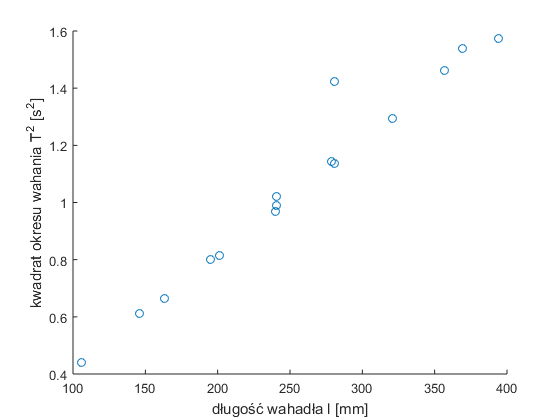
\includegraphics[scale=0.7]{wykres_punktowy}
		\caption{Wykres przedstawiający dane z tabeli \ref{tabela2}}
		\label{wykr1}
	\end{figure}
	Jesteśmy w stanie zauważyć na nim pomiar odbiegający od całej prostej pomiarów, uznajemy to za błąd gruby oraz nie uznajemy w dalszych obliczeniach. Dokładnie temu pomiarowi przyjrzymy się w podrozdziale \ref{analiza_niepewnosci}
	%----------------------------------------------------------------------------------------------------------	
	
	\subsection{Analiza niepewności}
	\label{analiza_niepewnosci}
	
%--------------------------------------------------------------------------------------------------------------

	\section{Podsumowanie}

%--------------------------------------------------------------------------------------------------------------
		
\end{document}